 
\chapter{Extension of the notion of Fourier transform}
\label{chap-extension-trans-fourier} 
 s
 
This chapter brings together many related notions of the Fourier transform, as well as direct applications of these developments. We will thus have to define new transformations, among others \textit{the Hartley transform}, the \textit{transform in Z}, and the \textit{fractional Fourier transform}. Most often, it is a question of finding algorithms to overcome certain weaknesses of the DFT (for example the \textit{Hartley transform}), or to extend certain notions in a natural way (the \textit{transformed into Z } for example). We will study in which cases these transformations are more efficient or more suitable than the discrete Fourier transform, and which applications can benefit from the fast algorithms obtained. The two important points to keep in mind when working with such transformations are: \begin{rs}
\item They do not correspond to approximate calculations. These are exact formulas, which very often have an inversion formula. These transforms can be useful for certain numerical computations (for example the approximate computation of a Fourier transform or of an infinite convolution), but they are above all algebraic calculations.
\item They have fast calculation algorithms. It is these algorithms which give all its value to a transform, and which make it usable in an intensive way. These algorithms are direct consequences of the algebraic nature of transforms, and only reflect certain algebraic symmetries and invariances.
\end{rs}
 
% ------------------------------------------------- -----
% ------------------------------------------------- -----
% ------------------------------------------------- -----
% section - Hartley transform                            
% ------------------------------------------------- -----
% ------------------------------------------------- -----
% ------------------------------------------------- -----
\section{Hartley transform}
% \addcontentsline{toc}{section}{Hartley transform}
\label{sect1-trans-hartley} 
 
\index{Hartley's!transform} \index{Hartley@\nompropreindex{Hartley}} One of the disadvantages of the discrete Fourier transform is that it requires calculations with complex numbers, which is not suitable for calculation of convolutions with real signals. Indeed, unnecessary complex multiplications and additions (more expensive than real multiplications and additions) are performed, and rounding errors are only amplified. We will define a transform, called \textit{Hartley transform}, which allows, like the DFT, to calculate convolution products, but which only involves calculations with real numbers. A very complete reference on the \textit{Hartley transform} and its applications is \nompropre{Bracewell} \cite{bracewell}.
% ------------------------------------------------- -----
% ------------------------------------------------- -----
% sub-section - Definition and first properties                            
% ------------------------------------------------- -----
% ------------------------------------------------- -----
\subsection{Definition and first properties}
 
 
 
\begin{defn}[Hartley transform]
\label{notation-58} \label{notation-59} Let $ f = \{f [n] \}_{n = 0}^{N-1} \in \CC^N $. We define its discrete \textit{Hartley transform} $ \Hh (f) \in \CC^N $ by
\begin{equation}
\label{eq-defn-transfo-hartley}
\forall k \in \{0, \ldots, \, N-1 \}, \quad \Hh (f) [k] \eqdef \sum_{n = 0}^{N-1}{f [n] \cas \left(\frac{2 \pi}{N} nk \right)},
\end{equation}
where we noted $ \cas (x) \eqdef \sin (x) + \cos (x) = \sqrt{2} \cos \left(x - \frac{\pi}{4} \right) $.
\end{defn}
 
 
\begin{rem}
The discrete Hartley transform has its continuous analogue, namely, for a function $ f \in L^1 (\RR) $, the function
\begin{equation*}
\Hh (f): s \rightarrow \int_{\RR}{f(x) \cas (2 \pi sx) \d x}.
\end{equation*}
Most of the statements valid in the discrete case have an analogous formulation for the continuous case, and it is left to the reader to state them.
\end{rem}
 
 
\begin{prop}[Inversion formula]
\label{prop-ptes-transfo-hartley}
\index{Inversion formula} $ \Hh $ is an isomorphism from $ \RR^N $ into $ \RR^N $. More precisely, for $ f \in \RR^N $, we have $ \Hh^2 (f) = N f $, which means that the inverse of the Hartley transform is $ \Hh^{-1} = \frac{1}{N} \Hh $.
\end{prop}
\begin{proofnoqed}
We will use, for $ n $ and $ n'\in \{0, \ldots, \, N-1 \} $, the orthogonality relation
\begin{equation}
\label{eq-orthogonalite-cas}
\sum_{k = 0}^{N-1}{\cas \left(\frac{2 \pi}{N} nk \right) \cas \left(\frac{2 \pi}{N} n' k \right)} = N \delta_n^{n'},
\end{equation}
where $ \delta_n^{n'} $ is 1 if $ n = n' $ and 0 otherwise. We denote by $ \omega = e^{\frac{2 \imath \pi}{N}} $, hence
\begin{equation*}
v_n [k] \eqdef \cas \left(\frac{2 \pi}{N} nk \right) = \frac{1}{2} \left(\omega^{nk} (1- \imath) + \omega^{- nk} (1+ \imath) \right).
\end{equation*}
We therefore calculate
\begin{equation}
\label{eqn-proof-inversion-hartley}
\dotp{v_n}{v_{n'}} = \frac{(1- \imath)^2}{4} \sum_{k}{\omega^{(n + n') k}} + \frac{(1+ \imath)^2}{4} \sum_{k}{\omega^{(n + n') k}} + \frac{(1- \imath) (1+ \imath)}{2} \sum_{k}{\omega^{(n-n') k}}.
\end{equation}
The first two sums are opposite, and the last is $ N \delta_{n}^{n'} $. To obtain the inversion formula, we note that $ \Hh (f) [n] = \dotp{f}{v_n} $, hence
\begin{equation*}
\Hh (\Hh (f)) [n] = \sum_{k = 0}^{N-1}{\Hh (f) [k] v_n [k]} = \sum_{k = 0}^{N-1}{f [k] \dotp{v_k}{v_n}} = N f [n]. \tag *{\qed}
\end{equation*}
\end{proofnoqed}
 
 
\begin{prop}
We have the following relations between the discrete Fourier transform and the Hartley transform of a vector $ f \in \RR^N $:
\begin{equation}
\label{eq-relation-tfd-hartley}
\begin{split}
\Hh (f) = & \realp (\Ff(f)) + \imagp (\Ff(f)) \\
\Ff(f) = & \psym{\Hh (f)} - \imath \pasym{\Hh (f)}.
\end{split}
\end{equation}
We have noted, for $ g \in \RR^N $, $ \psym{g} $ and $ \psym{g} $ the symmetric and anti-symmetric parts of $ g $, introduced in the definition \ref{defn-parts-sym-anti-sym}.
\end{prop}
 
 
\begin{rem}
The relations \eqref{eq-relation-tfd-hartley} imply, in the case where we restrict ourselves to real vectors, a one-to-one correspondence between discrete Fourier transform and Hartley transform. How to explain that $ N $ complex numbers (for the DFT) can contain as much information as only $ N $ real numbers? In reality, there is no contradiction, we just have to remember that in the case of a real signal, the vector $ \Ff(f) $ is the conjugate of $ \Ff(f^\sharp) $ (where $ f^\sharp $ is defined at the equation \eqref{eq-defn-symmetrical-sample}), there is therefore information redundancy (exactly twice as much information). For a real signal, the Hartley transform is much more economical (whether in terms of computation time or memory space) than the Fourier transform, since we will handle exactly half the information. It is this quality that we will exploit in the following paragraph.
\end{rem}
 
% ------------------------------------------------- -----
% ------------------------------------------------- -----
% sub-section - Fast Hartley transform                            
% ------------------------------------------------- -----
% ------------------------------------------------- -----
\subsection{Fast Hartley transform}
\label{sect2-algo-de-calcul-hartley} 
 
 
\index{Algorithm!FHT} \index{FHT} As for the DFT, we have a fast algorithm to calculate the Hartley transform. This algorithm has been described in detail by \nompropre{Ullmann} \cite{ullmann}. To understand it, we are going to perform a slicing of the transform, as we have already done during the study of the FFT algorithm. It is of course a question of exploiting the (algebraic) symmetries of the transformation, as well as the properties of the function $ \cas $. Once all this is in place, we will naturally see a recursive algorithm appear.
 
 
This algorithm uses a property of temporal decimation. To obtain the corresponding recurrence equation, we will proceed as we have already done for the discrete Fourier transform. We must decompose the sum that defines $ \Hh (f) $, for $ f \in \CC^N $, as follows:
\begin{equation}
\label{eq-decomposition-transfo-hartley1}
\Hh (f) [k] = \sum_{n = 0}^{N / 2-1}{f [2n] \cas \left(\frac{2 \pi}{N} 2 nk \right)} + \sum_{n = 0}^{N / 2-1}{f [2n + 1] \cas \left(\frac{2 \pi}{N} (2n + 1) k \right)}.
\end{equation}
Let us use the notations of \eqref{eq-part-even-odd}. We recognize in the left sum a Hartley transform of length $ N / 2 $, more precisely $ \Hh (f^{0}) $. The right sum poses a problem, but we can overcome this difficulty by using the following property of the function $ \cas $.
 
\begin{prop}
We have, for $ (\alpha, \, \beta) \in \RR^2 $,
\begin{equation}
\label{eq-prop-function-case}
\cas (\alpha + \beta) = \cas (\alpha) \cos (\beta) + \cas (- \alpha) \sin (\beta).
\end{equation}
\end{prop}
\begin{proof}
This property is demonstrated very simply by using the well-known trigonometric identities of the functions $ \cos $ and $ \sin $.
\end{proof}
Using this property, we can rewrite the second sum of the equation \eqref{eq-decomposition-transfo-hartley1} to get
\begin{equation*}
\Hh (f) [k] = \Hh (f^{0}) + \cos \left(\frac{2 \pi}{N} k \right) \Hh (f^{1}) [k] + \sin \left(\frac{2 \pi}{N} k \right) \Hh (f^{1}) [- k].
\end{equation*}
We then define the operator $ \chi_N^x $, for $ x \in \RR $, as follows:
\begin{equation}
\label{eq-decomposition-transfo-hartley2}
\forall a \in \CC^N, \quad \chi_N^xa \eqdef \left\{a [j] \cos \left(\frac{2 \pi jx}{N} \right) + a^{\sharp}[j] \sin \left(\frac{2 \pi jx}{N} \right) \right\}_{j = 0}^{N-1} \in \CC^N.
\end{equation}
We recall that $ a^{\sharp} $ is the symmetrized vector, equation \eqref{eq-defn-symmetrical-sample}. We are now going to split the vector $ \Hh (f) $ into its left and right parts, denoted $ \Hh (f)_g $ and $ \Hh (f)_d $. The relationship
\begin{equation*}
\cas \left(\frac{2 \pi}{N} (n + N / 2) \right) = - \cas \left(\frac{2 \pi}{N} n \right)
\end{equation*}
allows to obtain a very simple writing of the sought recurrence equation:
\begin{align}
\label{eq-decomposition-transfo-hartley}
\Hh (f)_g & = \Hh (f^0) + \chi_{N / 2}^{1/2} \Hh (f^1), \\
\label{eq-decomposition-transfo-hartley-2}
\Hh (f)_d & = \Hh (f^0) - \chi_{N / 2}^{1/2} \Hh (f^1).
\end{align}
These equations make it possible to immediately implement a fast calculation algorithm which we call \textit{FHT} for \textit{Fast Hartley Transform}. The \texttt{fht} procedure performs this algorithm by recursive calls, and its program can be found in Section~\ref{sect1-listing-fht}.
 
\begin{rem}
The recurrence equations \eqref{eq-decomposition-transfo-hartley} and \eqref{eq-decomposition-transfo-hartley-2} show that the computation of $ \Hh (f) $ actually requires the computation of two transforms of half size. However, because of the inverted term $ a^\sharp $ present in the operator $ \chi_N^x (a) $, it is difficult to use a butterfly scheme as for the FFT algorithm. In order to write an iterative algorithm, \nompropre{Ullmann}, in \cite{ullmann}, shows how we can do the computation by a double butterfly diagram, using four inputs.
\end{rem}
We can show that a butterfly transformation of the FHT algorithm requires four multiplications and six real additions. With regard to the FFT algorithm, we find one addition and two complex multiplications, ie four additions and six multiplications. However, the loop performed to calculate the butterfly transforms of the FFT algorithm runs from 0 to $ N-1 $, while for the FHT algorithm, it is a loop between 0 and $ N / 2-1 $. In the end, the FHT algorithm has the double advantage of requiring half the number of operations, and of using half the memory (we do not handle complex numbers).
 
\begin{rem}{(\upshape \textbf{Zero padding}).} 
\index{Zero padding} We have already explained in Paragraph~\ref{sect2-addition-zeros}, that it was possible to represent fairly faithfully the continuous DFT of a signal finished by \textit{zero padding}. It is of course possible to do the same with the Hartley transform. The FHT algorithm, combined with a zero-padding procedure, therefore makes it possible to simply calculate a continuous Hartley transform. The more zeros are added, the more intermediate values of the transform are calculated, and the better the calculation precision. The figure \figref{fig-comparison-fht-fft} shows this process on a simple (trianglular) signal, and allows to compare the Fourier spectrum (in fact its real part) and its Harley spectrum. Since the Hartley spectrum is the difference between the real and imaginary parts of the Fourier spectrum, the similarities are not accidental!\begin{figure}[ht]
    \begin{center}
    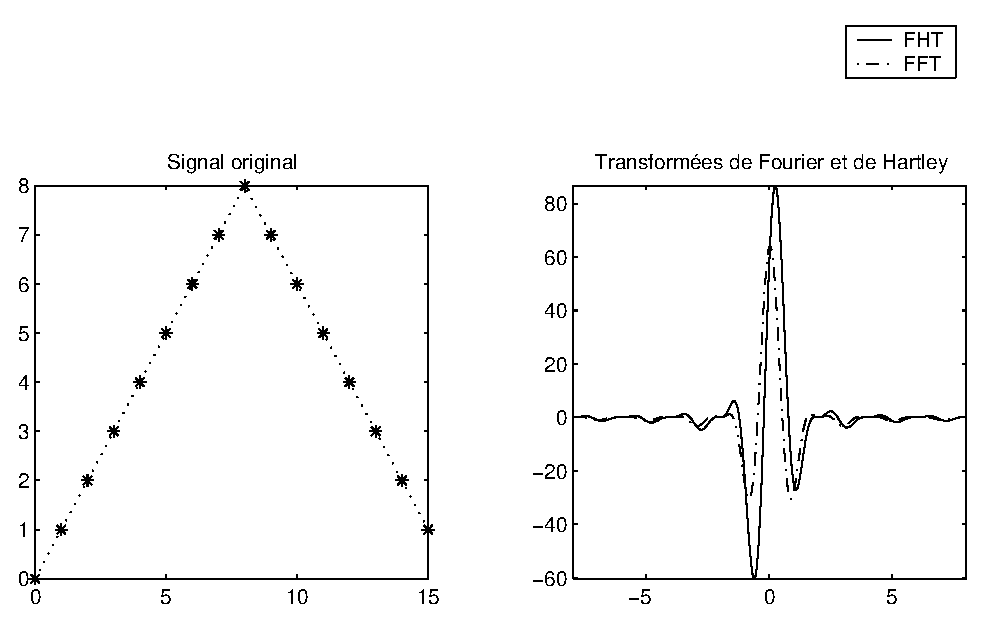
\includegraphics[scale=0.7]{images/comparaison-fht-fft.eps}
    \end{center}
    \caption{Comparison between the Hartley spectrum and the Fourier spectrum}
              \label{fig-comparison-fht-fft}
\end{figure}
\end{rem}
 
% ------------------------------------------------- -----
% ------------------------------------------------- -----
% sub-section - Calculation of convolution by Hartley transform                            
% ------------------------------------------------- -----
% ------------------------------------------------- -----
\subsection{Convolutional calculation by Hartley transform}
\label{sect2-usage-hartley-convolution} 
 
The equations \eqref{eq-relation-tfd-hartley} show that it is possible to calculate a DFT of a real signal by means of a Hartley transform calculation, which avoids having to resort to multiplications and complex additions. In the same vein, one can establish a formula which makes it possible to calculate a product of convolution of two real signals using only Hartley transforms.
 
\begin{prop}[Convolution and Hartley transform]
\index{Convolution!by Hartley transform} Let $ a $ and $ b $ be two real vectors of size $ N $. We have
\begin{equation*}
\Hh (a * b) = \frac{1}{2} \big \{\Hh (a) \Hh (b) - \Hh (a)^{\sharp} \Hh (b)^{\sharp } + \Hh (a) \Hh (b)^{\sharp} + \Hh (a)^{\sharp} \Hh (b) \big \},
\end{equation*}
that is, for $ n = 0, \ldots, \, N-1 $,
\begin{equation*}
\Hh (a * b) [n] = \frac{1}{2} \big \{c [n] (d [n] + d [-n]) + c [-n] (d [n] - d [-n]) \big \},
\end{equation*}
where we noted $ c \eqdef \Hh (a) $ and $ d \eqdef \Hh (b) $. We must of course consider the index $ -n $ as taken modulo $ N $.
\end{prop}
\begin{proofnoqed}
After inverting the summations in the expression of $ \Hh (a * b) [k] $ we find
\begin{equation*}
\Hh (a * b) [n] = \sum_{l = 0}^{N-1}{a [l] \sum_{k = 0}^{N-1}{b [k] \cas \left(\frac{2 \pi}{N} n (k + l) \right)}}.
\end{equation*}
Then it suffices to use the relation \eqref{eq-prop-function-case} to obtain
\begin{equation*}
\Hh (a * b) [n] = \Hh (b) [n] \sum_{l = 0}^{N-1}{a [l] \cos \left(\frac{2 \pi}{N} nk \right)} + \Hh (b)^{\sharp}[n] \sum_{l = 0}^{N-1}{a [l] \sin \left(\frac{2 \pi }{N} nk \right)}.
\end{equation*}
To conclude, all that remains is to express the functions $ \cos $ and $ \sin $ using the function $ \cas $ as follows:
\begin{equation*}
\left\{\begin{array}{l} \cos (x) = \cas (x) + \cas (-x) \\\sin (x) = \cas (x) - \cas (-x) \end{array} \right. . \tag *{\qed}
\end{equation*}
\end{proofnoqed}
The \listingterme{} \texttt{fht \_convol}, which can be found in the Section~\ref{sect1-listing-fht}, realizes this convolution of real signals using the FHT algorithm. It is more economical, both in terms of computation time, and in terms of memory space used.
 
\begin{rem}{(\upshape \textbf{Auto correlation}).} 
\index{Auto correlation} \index{Correlation} In the case where the signals $ a $ and $ b $ are equal, we can slightly optimize the implementation of the convolution calculation algorithm by writing
\begin{equation*}
\Hh (a * a) [k] = c [k] c [-k] + \frac{1}{2} (c [k]^2 - c [-k]^2).
\end{equation*}
\end{rem}
 
% ------------------------------------------------- -----
% ------------------------------------------------- -----
% ------------------------------------------------- -----
% section - Z transform and applications                            
% ------------------------------------------------- -----
% ------------------------------------------------- -----
% ------------------------------------------------- -----
\section{Z transform and applications}
% \addcontentsline{toc}{section}{Transformed to Z and applications}
\label{sect1-trans-Z} 
 
 
Our objective here is to give a relatively general framework to study transforms which have properties similar to those of the discrete Fourier transform, and in a way, generalize it (like for example the vector Z transform in Section~\ref{sect1-trans-Z-vector}, and the fractional Fourier transform in Section~\ref{sect1-transforme-fourier-fractionionnaire}). To do this, we will be interested in the generating functions, which we will call transform in Z. After the definition of this transform, we will present an immediate application of the transform in Z to the construction of filters defined by recurrence equations.
 
 
The work of \nompropre{Wich} \cite{wich} gathers a lot of information on the transform in Z. The link with generating series and holomorphic functions is discussed at length in the book of \nompropre{Demengel} \cite{demengel}.
% ------------------------------------------------- -----
% ------------------------------------------------- -----
% sub-section - Definition and formal properties                            
% ------------------------------------------------- -----
% ------------------------------------------------- -----
\subsection{Definition and formal properties}
\label{sect2-defn-trans-Z} 
 
Our goal is to make the link between transform in Z and whole series. We will therefore define the notion of transform in Z within the framework of signals of potentially infinite size. In practice, we will use the transform on signals of finite size, which allows us to not have to worry about possible convergence problems. We will therefore consider a sequence $ f = \{f [n] \}_{n \in \ZZ} \in \CC^{\ZZ} $. Only the study of the transfer function of a recursive filter (in Paragraph~\ref{sect2-application-trans-z-filters}) requires the use of an infinite series. However, even then we will have an exact expression of the transform (as a rational fraction), which will save us from any problems.
 
\begin{defn}[Transform to Z]
\index{Transform!in Z} \label{notation-60} Let $ f \in \CC^\ZZ $. We call \textit{transformed into Z} of $ f $ the function
\begin{equation}
\label{eq-trans-Z-defn}
\Zz (f): \func{D}{\CC}{z}{\sum_{n = \minf}^{\pinf}{f [n] z^{- n}}},
\end{equation}
where $ D $ is the (possibly empty) set of points where the series converges.
\end{defn}
 
 
\begin{rem}{(\upshape \textbf{Z transform and holomorphic functions}).} 
\index{Complete!series} \index{Laurent!series} \index{Generating!series} \index{Function!holomorphs} The theory of \textit{Laurent series} shows that the transform in Z is in fact defined at inside a crown of the type
\begin{equation*}
C_{\alpha}^{\beta} \eqdef \{z \in \CC; \; \alpha <| z | <\beta \} \quad \quad \text{for} 0 \leq \alpha <\beta,
\end{equation*}
where $ \beta $ can optionally be $ + \infty $. We can refer for example to the book of \nompropre{Cartan} \cite{cartan-holo} for a complete study of the decomposition of a holomorphic function in integer series and in Laurent series. The function $ \Zz (f) $ is therefore holomorphic inside its convergence disk. It is also often said that $ \Zz (f) $ is the generating series associated with the sequence $ f $. As we will see later (by considering recursive filters), this notion makes it possible to represent in an elegant way certain sequences which are defined by induction. For an interesting talk on the resolution of recurrences by generating series, we can look at the reference work of \nompropre{Donald Knuth} \cite{knuth-concrete}. A simpler discussion can be found in \cite{froidevaux}. The book \cite{generatingfunctionology} is an original work on the subject.
\end{rem}
 
 
\begin{exmp}
Here are some simple examples. \begin{enumerate}
\item Let the sequence $ f \in \CC^\ZZ $ be defined by $ f [n] \eqdef 0 $ for $ n <0 $ and $ f [n] \eqdef 1 $ otherwise. We have
\begin{equation*}
\Zz (f) (z) = \sum_{n \geq 0}{z^{- n}} = \frac{1}{1-z^{-1}},
\end{equation*}
the series being convergent in $ C_1^{\pinf} $.
\item For $ (a, \, b) \in \CC^2 $, we define the sequence $ f \in \CC^\ZZ $ by $ f [n] \eqdef a^n $ for $ n \ge 0 $ and $ f [n] \eqdef b^n $ otherwise. We have
\begin{equation*}
\Zz (f) (z) = \sum_{n \geq 0}{\left(\frac{a}{z} \right)^n} + \sum_{n \geq 0}{\left(\frac{z}{b} \right)^n} - 1 = \frac{1}{1 - a / z} + \frac{1}{1 - z / b} - 1,
\end{equation*}
the sum being convergent in $ C_{| a |}^{| b |} $.
\end{enumerate}
\end{exmp}
 
 
\begin{prop}[Properties of the Z transform]
\label{prop-prte-z-trans}
We denote by $ f $ and $ g $ two sequences of $ \CC^\ZZ $. Besides linearity, here are the important properties of the Z transform: \begin{itemize}
\item [{\upshape (i)}] linear convolution:
\begin{equation*}
\Zz (f \star g) = \Zz (f) \Zz (g),
\end{equation*}
the series defining $ \Zz (f \star g) $ being at least convergent on the intersection of the convergence rings of $ \Zz (f) $ and $ \Zz (g) $ (if it is not empty).
\item [{\upshape (ii)}] derivation:
\begin{equation*}
\Zz \left(\{nf [n] \}_{n \in \ZZ} \right) (z) = - z \frac{d}{dz} \Zz (f) (z).
\end{equation*}
\end{itemize}
\end{prop}
\begin{proof}
We will prove the most important property, the convolution property (i). The absolute convergence on the intersection of the convergence domains allows us to write, for $ z $ in this intersection:
\begin{equation*}
\begin{split}
\Zz (f \star g) (z) & = \sum_{n = \minf}^{\pinf}{\left(f \star g [n] \right) z^{- n}} = \sum_{n = \minf}^{\pinf}{\sum_{m = \minf}^{\pinf}{f [n] g [nm] z^{- n}}} \\
& = \sum_{m = \minf}^{\pinf}{f [m] z^{- m}} \left(\sum_{n = \minf}^{\pinf}{g [nm] z^{- (nm)}} \right) \\
& = \Zz (f) (z) \Zz (g) (z).
\end{split}
\end{equation*}
Absolute convergence justifies the inversion of the two summations.
\end{proof}
 
 
\begin{rem}
There are also formulas allowing to integrate the function $ \Zz (f) $. They require the use of curvilinear integrals, as well as possible precautions on the behavior at infinity of $ f $.
\end{rem}
 
% ------------------------------------------------- -----
% ------------------------------------------------- -----
% sub-section - Recursive filters                            
% ------------------------------------------------- -----
% ------------------------------------------------- -----
\subsection{Recursive filters}
\label{sect2-application-trans-z-filters} 
 
 
We have already seen in Section~\ref{sect1-filtering}, the definition of linear filters, as well as their use to modify signals appropriately. We are going to define here a new type of filters, named \textit{recursive filters}, which also allow us to perform interesting operations on signals. The Z transform is very often used to represent the transfer function of recursive filters. It is indeed very practical for at least two reasons: \begin{rs}
\item the representation in the form of a function will allow the use of algebraic operations to modify the filter (sum, product, derivative, etc.).
\item the complex representation in the form of module and argument (that is to say in polar coordinates) will allow you to create filters from scratch in an intuitive way.
\end{rs}
 
 
Excellent books are available on digital signal processing in general, and using the Z transform for creating filters. We can cite among others \cite{smith-segdps} as well as \cite{claerbout-fgdp}.
 
 
 
 
\begin{defn}[Recursive filter]
\index{Filter!recursive} \label{notation-61} Let $ a = \{a_0, \ldots, \, a_k \} $ and $ b = \{b_1, \ldots, \, b_l \} $ two vectors of complex numbers. They allow to define the \textit{recursive filter} $ \Phi_a^b $ operating on sequences $ x \in \CC^{\NN} $ by defining $ y = \Phi_a^b (x) \in \CC^{\NN} $ by
\begin{equation}
\label{eq-defn-recursive-filter}
\begin{split}
\forall n \in \ZZ, \quad y [n] = a_0 x [n] & + a_1 x [n-1] + \cdots + a_k x [nk] \\
& + b_1 y [n-1] + \cdots + b_l y [nl].
\end{split}
\end{equation}
\end{defn}
 
 
\begin{rem}
\index{Support} \index{Filter!causal} \index{Causality} The equation \eqref{eq-defn-recursive-filter} therefore defines the filter by induction. The filter uses, for the computation of $ y [n] $, only already computed values of $ y $ as well as inputs of the vector $ x $ of index less than $ n $. In accordance with the terminology already used (for convolutional filters), we say that the filter is causal. We thus obtain a simple algorithm to evaluate the action of the filter on a signal $ x $. In the following, only $ x $ filters with finite support will be considered, and all the signals involved (in particular $ x $ and $ y $) will be indexed from zero. Note that the computation of the first inputs of the vector $ y $ requires the knowledge of $ y [-1], \, y [-2], \ldots, \, y [-l] $, as well as $ x [n -1], \, x [n-2], \ldots, \, x [-k] $. By convention, it will be assumed, unless explicitly stated to the contrary, that these entries are null.
\end{rem}
 
 
\begin{rem}{(\upshape \textbf{Link with convolution filters}).} 
\index{Filter!of convolution} We have already defined, in Section~\ref{sect1-filtering}, finite convolution filters. Note that in the case where the vector $ b $ is zero, the recursive filter is in fact a finite convolution filter. Recursive filters can be seen, from a theoretical point of view, as a generalization of linear convolution filters. In fact, we will see even in the following study, by the calculation of the transform in Z, that the recursive filters are filters of convolution, but of which the impulse response is infinite. This is why they are called \textit{IIR} filters in the English literature (abbreviation of \textbf{I} nfinite \textbf{I} mpulse \textbf{R} esponse). From a pragmatic point of view, it is not the same: the uses of these two types of filtering are different, mainly because of the properties inherent both in their implementation, and in their impulse responses. Unlike a linear convolutional filter which can be computed quickly by FFT, a recursive filter will generally be limited to only a few recurrence terms (meaning that $ k $ and $ l $ will often be assumed to be small). These filters therefore make it possible, without having to calculate convolutions, to obtain very long responses (in theory infinite) for very low costs, of the order of $ \grdo (N) $ (where $ N $ denotes the size filtered vectors), assuming that $ k $ and $ l $ are small in front of $ N $. On the other hand, the fact of having only a small number of coefficients at its disposal to create these filters makes them less manageable. Finally, it should be noted that the calculation of a filter by induction facilitates the propagation of rounding errors (since they are added as the calculations progress). To stop this phenomenon, we are often obliged to do double precision calculations.
\end{rem}
 
 
 
The idea of this paragraph is to use the Z transform to define a recursive filter in a nicer way than by the recurrence equation \eqref{eq-defn-recursive-filter}. To do this, let's calculate the Z transform of this equation. After grouping the terms, we get
\begin{equation*}
\Zz (y) (z) = H (z) \Zz (x) (z),
\end{equation*}
with
\begin{equation*}
H (z) \eqdef \frac{a_0 + a_1 z^{-1} + \cdots + a_k z^{- k}}{1 - b_1 z^{-1} - \cdots - b_l z^{- l }}.
\end{equation*}
We want to assert that $ H $ is the transform in Z of a certain transfer function $ h $, in order to write the filter $ \Phi_a^b $ as being the convolution filter $ \Phi_h $. Indeed, suppose that we succeeded in finding such a $ h $. Using the convolution result \ref{prop-prte-z-trans} (i), we get
\begin{equation*}
\Zz (y) = H \cdot \Zz (x) = \Zz (h \star x) = \Zz (h) \cdot \Zz (x).
\end{equation*}
\index{Formula!of Cauchy} \index{Cauchy@\nompropreindex{Cauchy}} We can see that $ H = \Zz (h) $. The problem is to know if knowing $ H $ makes it possible to determine such $ h $, in other words, if it is possible to calculate the inverse of the transform in Z. The answer is far from obvious. We know, thanks to \textit{Cauchy formulas}, that a holomorphic function defined on a crown $ C_{\alpha}^{\beta} $ admits a unique series expansion of Laurent inside this crown. However, it remains to be seen which crown we are dealing with. According to the choice of the domain of convergence, one obtains a sequence $ h $ different. So we need more information about the filter. By taking the Z transform of the recurrence equation \eqref{eq-defn-recursive-filter}, we kind of have \guill{forgot} the boundary conditions, i.e. the values of $ x [-1], \ldots, \, x [-k] $ as well as $ y [-1], \ldots, \, y [-l] $. In practice, we have in fact simple information which makes it possible to find the domain of convergence which corresponds to the recurrence equation, and thus to find the sequence $ h $ starting from $ H $. \begin{rs}
\item \index{Filter!causal} \index{Causality} If we consider the recurrence equation written in \eqref{eq-defn-recursive-filter}, we see that the considered filter is causal (i.e. - say that the determination of $ y [n] $ depends only on entries with indices less than $ n $ of $ x [n] $). This implies that the impulse response is zero for negative indices, which results in the fact that the domain of convergence is outside a circle (it suffices to use the convergence criterion for a whole series, since l'we actually have an entire series in $ 1 / z $).
\item Most often, we want the filter to be stable in addition to being causal, which implies, as we will see in the proposition \ref{prop-poles-stability}, that the domain of convergence must contain the unit circle.
\end{rs} Here is an example that shows the importance of specifying the domain of convergence.
 
\begin{exmp}[Causality and domain of convergence]
\index{Filter!causal} \index{Causality} We consider a signal $ y $ which satisfies the difference equation
\begin{equation}
\label{eq-recurrence-1st-order}
y [n] = \alpha y [n-1] + x [n],
\end{equation}
where $ x \in \CC^\ZZ $ is the input signal. One thus obtains for the impulse response the transform in Z following:
\begin{equation*}
H (z) = \frac{1}{1 - \alpha z^{-1}}.
\end{equation*}
In a natural way, the equation \eqref{eq-recurrence-1st-order} defines a causal filter, and we can try to find its impulse response by the method we have just explained. The function $ H $ must therefore be considered as defined outside the circle of radius $ | \alpha | $. We then obtain, by expanding the whole series fraction as a function of $ z^{-1} $,
\begin{equation*}
\forall z \in C_{| \alpha |}^{\pinf}, \quad H (z) = \sum_{n \geq 0}{\alpha^nz^{- n}}.
\end{equation*}
Hence the value of the impulse response $ h $:
\begin{equation*}
\begin{split}
\forall n <0, \quad h [n] & = 0, \\
\forall n \geq 0, \quad h [n] & = \alpha^n.
\end{split}
\end{equation*}
It is therefore indeed a causal filter. If we want it to be stable, we check that we must also assume that $ | \alpha | <$ 1. However, another case can occur, if we consider that the function $ H $ is defined on $ C_0^{| \alpha |} $. This time you have to do the following:
\begin{equation*}
\forall z \in C_{0}^{| \alpha |}, \quad H (z) = \frac{- z / \alpha}{1 - z / \alpha} = \sum_{n <0}{- \alpha^nz^{- n}}.
\end{equation*}
We thus obtain the expression of $ h $:
\begin{equation*}
\begin{split}
\forall n <0, \quad h [n] & = - \alpha^n, \\
\forall n \geq 0, \quad h [n] & = 0.
\end{split}
\end{equation*}
The filter is therefore anti-causal, and stability dictates that $ | \alpha | > $ 1. The fact that it is anti-causal can be explained simply by rewriting the recurrence equation \eqref{eq-recurrence-1st-order} in an inverse form (propagation of calculations in the other direction):
\begin{equation*}
y [n-1] = \frac{1}{\alpha} y [n] - \frac{1}{\alpha} x [n].
\end{equation*}
\end{exmp}
Once we have succeeded in obtaining the value of $ h $, we see that the filter $ \Phi_a^b $ is indeed a convolution filter, but which remains a little special, since its impulse response, in the domain of the transform in Z, can be put in the form of a rational fraction.
 
 
We have just seen how we can represent the transfer function of a recursive filter thanks to its Z transform. This representation has the advantage of offering a compact and simple writing. This allows efficient calculations on filters, more simply than allowed by the representation in the form of convolution exposed in Paragraph~\ref{sec2-linear-filters}. Before studying the use of the Z transform for the creation of new filters, let's see the relationship between the rational fraction representing a filter, and the stability of this filter.
 
\begin{prop}[Poles and stability]
\label{prop-poles-stability}
\index{Pole} \index{Stability} Let $ H (z) = \frac{A (1 / z)}{B (1 / z)} $ be the Z transform of the transfer function of a filter $ \Phi_a^b $ (which is therefore causal). Then, this filter is stable if and only if all the poles of $ H $ are located inside the unit circle $ \Gamma $.
\end{prop}
\begin{proof}
\index{Causality} \index{Filter!causal} We have already said that for a causal filter, the series that defines $ H $ converges outside a certain circle, and the converse is true (it suffices to consider the expansion in $ 1 / z $ of a holomorphic function defined in the neighborhood of infinity). Since $ \Phi_a^b $ is of course causal, this remark applies. In addition, we saw in Paragraph~\ref{sect2-responses-stability}, that an impulse response filter $ h $ was stable if and only if $ \norm{h}_{\ell^1} <+ \infty $. If $ h $ is absolutely summable, we have the markup
\begin{equation*}
\forall z \in \Gamma, \quad | H (z) | \leq \sum_{n = \minf}^{\pinf}{| h [n] z^{- n} | } = \sum_{n = \minf}^{\pinf}{| h [n] | } \eqdef \norm{h}_{\ell^1}.
\end{equation*}
We thus see that the condition $ \norm{h}_{\ell^1} <+ \infty $ implies that the series which defines $ H $ is absolutely convergent on the circle $ \Gamma $. The converse is true. The fact that $ \norm{h}_{\ell^1} <+ \infty $ is therefore equivalent to the fact that the convergence region contains everything outside the circle $ \Gamma $. However, the region of convergence cannot contain a pole. All the poles of the rational fraction $ H $ must therefore have a modulus strictly less than 1. Once again, the converse is true.
\end{proof}
 
% ------------------------------------------------- -----
% ------------------------------------------------- -----
% sub-section - Application to the construction of filters                            
% ------------------------------------------------- -----
% ------------------------------------------------- -----
\subsection{Application to the construction of filters}
 
 
In this paragraph, we will focus on using the Z transform for the creation of digital recursive filters. The process for creating a filter is to decide where the zeros and poles of the transfer function are located. As we have already seen, the poles must be contained in the unit circle for the filter to be causal and stable. For example, we can choose the locations identified in the figure \figref{fig-location-poles-notch-filter}, which leads to the expression of the transfer function:
\begin{equation*}
H (z) = \frac{(z - e^{\imath \pi / 4}) (z - e^{- \imath \pi / 4})}{(z - 0.9 e^{\imath \pi / 4}) (z - 0.9 e^{- \imath \pi / 4})} \approx \frac{1 - 1.414 z + z^2}{0.810 - 1.273 z -z^2}.
\end{equation*}
\begin{figure}[ht] 
    \begin{center}
    \includegraphics[scale=0.5]{images/emplacement-poles-notch-filter.eps}
    \end{center}
    \caption{Positioning of poles and zeros}
              \label{fig-location-poles-notch-filter}
\end{figure}
This Z transform is shown in figure \figref{fig-notch-filter-trans-z}. From this expression, we immediately deduce the coefficients of the associated recursive filter:
\begin{equation*}
\begin{array}{ccc} a_0 = 1 & a_1 \approx -1.414 & a_2 = 1 \\b_0 \approx 1.273 & b_1 \approx -0.810. & \end{array}
\end{equation*}
Therefore, if we want to calculate the frequency response, two methods are available to us: \begin{rs}
\item \index{Frequency response} calculate the frequency response directly from $ H $: it suffices to consider the value of the transfer function on the unit circle, i.e. the function $ \xi \mapsto H (e^{2 \imath \pi \xi}) $, for $ \xi \in [0,1] $. By inverse Fourier transform, the impulse response is deduced therefrom (the approximate calculation is done by sampling the frequency response, then by inverse FFT).
\item calculate the impulse response using the filter recurrence equation and applying it for the impulse $ \delta_0 $. We can then use a (discrete) Fourier transform to approximate the frequency response. To have sufficient precision, it will be necessary to calculate a fairly long approximate impulse response.
\end{rs} Figure \figref{fig-notch-filter-rep-imp-freq} shows the impulse and frequency responses of the filter. They were calculated directly from the transfer function $ H $ shown in figure \figref{fig-notch-filter-trans-z}. In paragraph \ref{sect2-algo-trans-z}, we will present a fast calculation algorithm to determine the value of the Z transform on some contours, and we will calculate the impulse response from the recurrence equation \eqref{eq-defn-recursive-filter}. \begin{figure}[ht]
    \begin{center}
    \includegraphics[scale=0.5]{images/notch-filter-trans-z.eps}
    \end{center}
    \caption{Z transform of the filter}
              \label{fig-notch-filter-trans-z}
\end{figure}
\begin{figure}[ht] 
    \begin{center}
    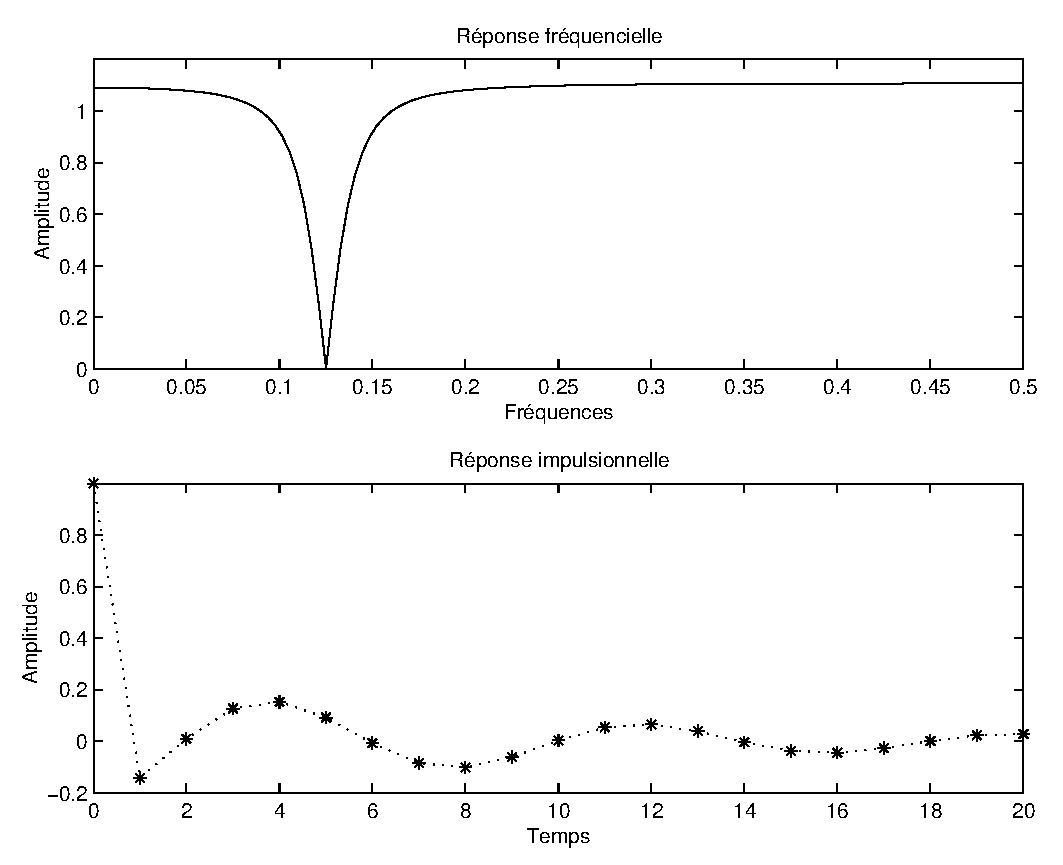
\includegraphics[scale=0.5]{images/notch-filter-rep-imp-freq.eps}
    \end{center}
    \caption{Frequency and impulse response of the filter}
              \label{fig-notch-filter-rep-imp-freq}
\end{figure}
 
 
 
The previous example is far from being as anecdotal as it seems. Indeed, by breaking down the rational fraction $ H $, we will be able to reduce ourselves to the case of simple filters, that is to say with at most two poles and two zeros. Here are two steps we can take. \begin{rs}
\item \index{Decomposition!into products} \index{Factorization} \index{Polynomial!irreducible} \textbf{Decomposition into products.} We can factorize the numerators and denominators into polynomials of degree 1 or 2 on $ \RR [ X] $ (respectively of degree 1 over $ \CC [X] $). We thus obtain the writing of the filter $ \Phi_a^b $ in the form of a cascade of filters:
\begin{equation*}
\Phi_a^b = \Phi_{\alpha_1}^{\beta_1} \circ \cdots \circ \Phi_{\alpha_p}^{\beta_p},
\end{equation*}
where each $ \alpha_i $ and $ \beta_i $ represents the coefficients of a polynomial of degree at most 2 (respectively at most 1). The filter $ \Phi_a^b $ therefore corresponds to the serialization of a series of recursive filters of order at most 2 (respectively at most 1).
\item \index{Decomposition!into simple elements} \index{Simple element} \textbf{Decomposition into simple elements.} We can decompose the fraction $ H $ into the sum of simple elements over $ \RR [X] $ (respectively $ \CC [X] $). We then obtain the decomposition
\begin{equation*}
\Phi_a^b = \Phi_{\alpha_1}^{\beta_1} + \cdots + \Phi_{\alpha_p}^{\beta_p},
\end{equation*}
where each $ \alpha_i $ and $ \beta_i $ represents the coefficients of a polynomial of degree at most 2 (respectively at most 1).
\end{rs} In the case where we carry out decomposition on $ \CC [X] $, even if the signals are real, we will have to do the convolution calculations with complex numbers. Each of these decompositions provides a new way to implement the recursive filter, in addition to the naive implementation of the \eqref{eq-defn-recursive-filter} equation. The \oldref{exo-calcul-spline-iir} exercise applies these two methods to calculate the coefficients of an interpolation by splines.

% ------------------------------------------------- -----
% ------------------------------------------------- -----
% sub-section - Reconciliation with analog filtering                            
% ------------------------------------------------- -----
% ------------------------------------------------- -----
\subsection{Reconciliation with analog filtering}
 
 
\index{Filter!analog} \index{Signal} Before going into the details of the implementation of a discrete Z transform, we will try to establish a connection between the digital recursive filters and the analog filters. Analog filters are in a way the ancestors of modern digital filters, but are still used in many situations. It is therefore interesting to understand why recursive filters (which perform discrete transformations) make it possible to replace analog filters (which perform continuous transformations) within the \guill{modern} framework of digital signal processing. Without going into the description of analog filtering, let's just say that it's a matter of passing a DC signal through a set of electronic components, so that the output signal is linked to the input signal by a linear differential equation. The digital filter then behaves like a dynamic system governed by a differential equation.
 
 
\index{System!dynamic} \index{Equation!with differences} \index{Equation!differential} \index{Circuit RLC} The difference equation \eqref{eq-defn-recursive-filter} is in fact the analog discrete of the differential equations that dynamical systems must satisfy. We can take the example of a \textit{circuit RLC} (see the diagram in figure \figref{fig-circuit-rlc}). We then have the following differential equation which connects $ V_e $ and $ V_s $, the input and output voltages:
\begin{equation}
\label{eq-equation-circuit-rlc}
\frac{d V_e}{dt} = \frac{1}{RC} V_s + \frac{d V_s}{dt} + \frac{L}{R} \frac{d^2 V_s}{dt^2 }.
\end{equation}
\begin{figure}[ht] 
    \begin{center}
    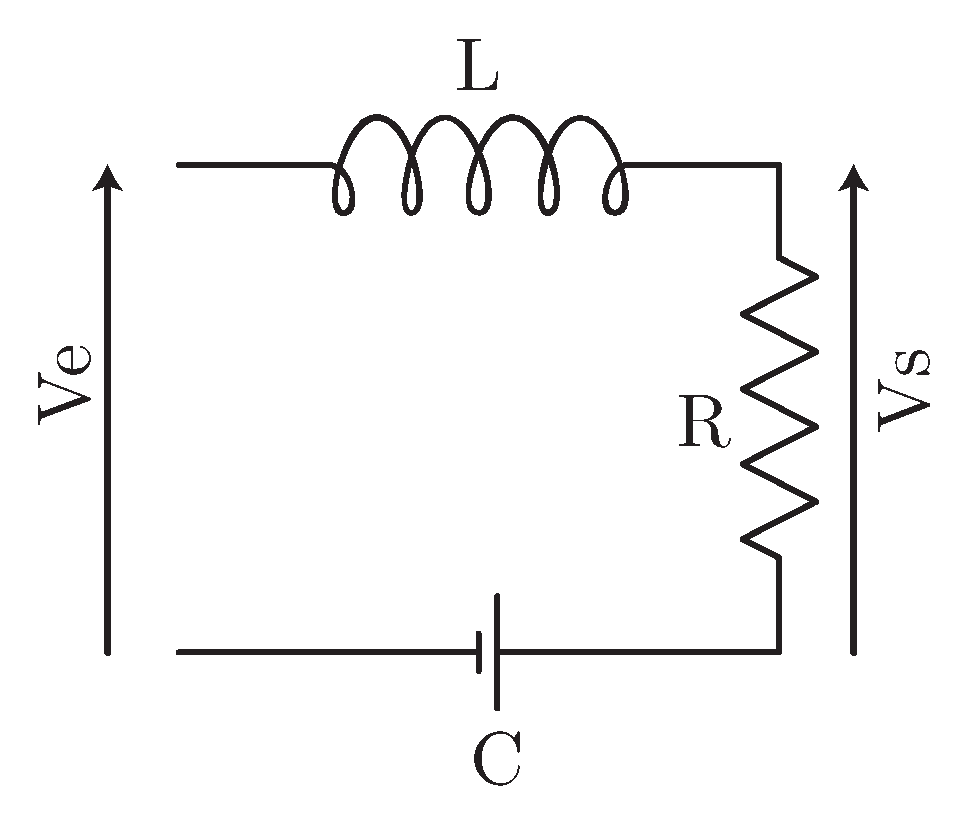
\includegraphics[scale=0.4]{images/circuit-rlc.eps}
    \end{center}
    \caption{RLC circuit}
              \label{fig-circuit-rlc}
\end{figure}
\index{Filter!analog} We can consider this circuit as an analog filter. As we have developed the Z transform to study discrete filters, we will introduce another generalization of the Fourier transform, continued this time, to study analog filters. This is the \textit{Laplace transform}, which is defined as follows.
 
\begin{defn}[Laplace transform]
\index{Laplace!transform} \index{Laplace@\nompropreindex{Laplace}} \label{notation-62} For a function $ f: \RR \rightarrow \CC $, we formally define its \textit{Laplace transform } through
\begin{equation*}
\forall s \in D, \quad \Ll(f) (s) \eqdef \int_{t \in \RR}{f(t) e^{- st} \d t}.
\end{equation*}
The function $ \Ll(f) $ is defined on a domain $ D $ where the integral converges.
\end{defn}
By taking precautions on the fields of definition of the functions considered, one can define the transfer function of the analog filter, in the field of Laplace:
\begin{equation*}
K (s) \eqdef \frac{\Ll(V_s) (s)}{\Ll(V_e) (s)} = \frac{s}{\frac{1}{RC} + s + \frac{L }{R} s^2}.
\end{equation*}
We have simply calculated the Laplace transform of the two members of the equation \eqref{eq-equation-circuit-rlc} here. We used the fact that the Laplace transform transforms the derivation into the multiplication by the parameter $ s $.
 
 
We are now interested in the problem resulting from the discretization, at regular time intervals $ \Delta $, of the studied signals. We obtain discrete signals $ \wt{V_e} $ and $ \wt{V_s} $, which satisfy the difference equation
\begin{align*}
\frac{1}{\Delta} \left(\wt{V_e}[n] - \wt{V_e}[n-1] \right) & = \frac{1}{RC} \wt{V_s}[ n] + \frac{1}{\Delta} \left(\wt{V_s}[n] - \wt{V_s}[n-1] \right) \\
& + \frac{L}{R \Delta^2} \left(\wt{V_s}[n] + \wt{V_s}[n-2] - 2 \wt{V_s}[n-1] \right).
\end{align*}
The resolution of the original differential equation is thus replaced by an explicit finite difference scheme. Of course, one could have chosen other methods to calculate in an approximate way the derivatives involved. That would have led to a slightly different equation. The exercise \oldref{exo-meth-quadratures-recursive-filter} proposes to calculate some finite difference equations for an integrating analog circuit.
 
 
From a purely discrete point of view, we obtain a recursive filter, which can be calculated using a computer (and no longer an electrical circuit as was the case for the RLC filter). We can then calculate the transfer function in the domain of the Z transform to study this filter:
\begin{equation*}
H (z) \eqdef \frac{1 - z}{\left(\frac{\Delta}{RC} + 1 + \frac{L}{\Delta R} \right) - \left(1 + \frac{2 L}{R \Delta} \right) z - \frac{2 L}{R \Delta} z^2}.
\end{equation*}
The Z transform is in a way the tool that allows us to study recursive filters, while the Laplace transform allows us to study their continuous cousins, the analog filters. Thus, the principles of construction of digital filters by the use of the transform in Z (placement of poles and zeros, placing in series of filters, etc.) also apply to the creation of analog filters, provided that use the Laplace transform.
% ------------------------------------------------- -----
% ------------------------------------------------- -----
% ------------------------------------------------- -----
% section - Transformed into vector Z                            
% ------------------------------------------------- -----
% ------------------------------------------------- -----
% ------------------------------------------------- -----
\section{Vectorial Z Transform}
% \addcontentsline{toc}{section}{Transformed to vector Z}
\label{sect1-trans-Z-vector} 
 
\index{Sampling} The presentation we have just made of the Z transform is above all theoretical. In order to actually calculate the values of a transformed function in Z, we need to sample and do a finite number of calculations. This is what we will do in this paragraph, by defining a new transform, which we call Z \textit{vector} transform. The resulting algorithm is called the \textit{chirp} algorithm. It was discovered for the first time, in the (more restricted) framework of the TFD by \nompropre{Bluestein}, and is well explained in the article \cite{swarztrauber-bluestein}. Some aspects of programming the Z transform are discussed in \cite{arndt-algo-programmers}.
% ------------------------------------------------- -----
% ------------------------------------------------- -----
% sub-section - Discrete calculation algorithm                            
% ------------------------------------------------- -----
% ------------------------------------------------- -----
\subsection{Discrete calculation algorithm}
\label{sect2-algo-trans-z} 
 
 
\index{Maple@\Maple{}} \index{Matlab@\Matlab{}} The Z transform, even operating on discrete and finite samples, nonetheless remains a function of the complex variable $ z $. The fact is that a computer does not know how to work directly with such functions (except for software such as \textsc{Maple} which can do certain formal operations). We therefore need a way to numerically evaluate the value of the Z transform at certain points, and this quickly. To build this algorithm, we will introduce a transform dedicated to the computation of $ \Zz (f) $ in a sufficient number of points (as many as there are points in the original sample).
 
\begin{defn}[Transform to vector Z]
\label{notation-63} \index{Transformed!into vector Z} We fix $ z \in \CC $. For a vector $ f \in \CC^N $, we define the \textit{transformed into vector Z} (at the point $ z $) by
\begin{equation}
\label{eq-defn-z-transform-vector}
\Gg_z (f) \eqdef \{\Zz (f) (z^n) \}_{n = 0}^{N-1} = \left\{\sum_{k = 0}^{N-1 }{f [k] z^{- kn}} \right\}_{n = 0}^{N-1}.
\end{equation}
\end{defn}
 
 
\begin{rem}
The vector obtained can be seen as the calculation of the value that the Z transform takes along a curve drawn in the complex plane. If the point $ z $ is taken from modulus 1, this curve will be the unit circle, otherwise, it will be a spiral.
\end{rem}
 
 
 
\index{Algorithm!CZT} \index{CZT} \index{Chirp} Let $ z \in \CC $ fixed. To build an efficient computation algorithm for $ \Gg_z (f) $, we will use the relation
\begin{equation*}
\forall (n, \, k), \quad nk = \frac{1}{2} \left(n^2 + k^2 - (nk)^2 \right).
\end{equation*}
Applying it to the definition equation \eqref{eq-defn-z-transform-vector}, we get
\begin{equation*}
\Gg_z (f) [n] = z^{- \frac{n^2}{2}} \sum_{k = 0}^{N-1}{f [k] z^{- \frac{k^2}{2}} z^{\frac{(nk)^2}{2}}} = z^{- \frac{n^2}{2}} (\wt{f} \star g) [not],
\end{equation*}
where we denote by $ g $ the vector defined by
\begin{equation*}
\forall k \in \{- N + 1, \, N-1 \}, \quad g [k] \eqdef z^{- \frac{k^2}{2}},
\end{equation*}
and $ f $ the vector
\begin{equation*}
\forall k \in \{0, \ldots, \, N-1 \}, \quad \wt{f}[n] \eqdef f [k] z^{- \frac{k^2}{2} }.
\end{equation*}
\index{Convolution!circular} Be careful that convolution is a linear convolution between a vector of size $ N $ and a vector of size $ 2N-1 $. Using the method described in Section~\ref{sect1-convolution-acyclic}, one can compute an acyclic convolution very quickly by replacing it with a larger cyclic convolution. More precisely, the vectors to be combined being of size $ N $ and $ 2N-1 $, it is in theory necessary to calculate a cyclic convolution of size $ 3N-2 $. \index{Cooley-Tukey@\nompropreindex{Cooley-Tukey} } In fact, to use a Cooley-Tukey \guill{classic} FFT algorithm, we add zeros to reach a size $ M = 2^k $ just after $ 3N-2 $. However, we can do much better (size $ 2N-1 $) by exploiting the fact that $ g [k] = g [-k] $. This is explained in the exercise \oldref{exo-chirp-transform-toeplitz} and gives rise to the procedure \Matlab{} \texttt{czt} (for \textbf{C} hirp \textbf{Z} \textbf{T } ransform) (see the correction of the exercise \oldref{exo-chirp-transform-toeplitz}). We can thus calculate the vector Z transform in a time of the order of $ \grdo (N \log (N)) $.
 
 
The \guill{chirp} approach therefore consists in replacing a transform calculation by a convolution calculation. Another trick (using a finite field) allows you to achieve a similar result (when $ N $ is a prime number). This is the subject of the exercise \oldref{exo-chirp-transform-finis-corps}.
 
 
\index{Pole} To finish, let's use the computation algorithm we just built to draw vector Z transforms of a recursive filter. We have chosen the filter whose poles and zeros are placed on the figure \figref{fig-location-poles-notch-filter}. We calculated the impulse response of the filter by directly using the recurrence equation \eqref{eq-defn-recursive-filter}. We have chosen two contours, which correspond respectively to $ z = e^{\frac{2 \imath \pi}{N}} $ (unit circle) and $ z = 1.001 e^{\frac{2 \imath \pi }{N}} $ (spiral). The first contour is used to calculate the impulse response (we find the figure \figref{fig-notch-filter-rep-imp-freq}). Indeed, calculating the transform in Z for $ z = e^{\frac{2 \imath \pi}{N}} $ amounts to calculating a DFT (with a substantial time saving if $ N $ is not a power of 2). For the second contour, on the other hand, we see that the second \guill{jump} is less marked, because the spiral is farther from the second pole than the unit circle is. \begin{figure}[ht]
    \begin{center}
    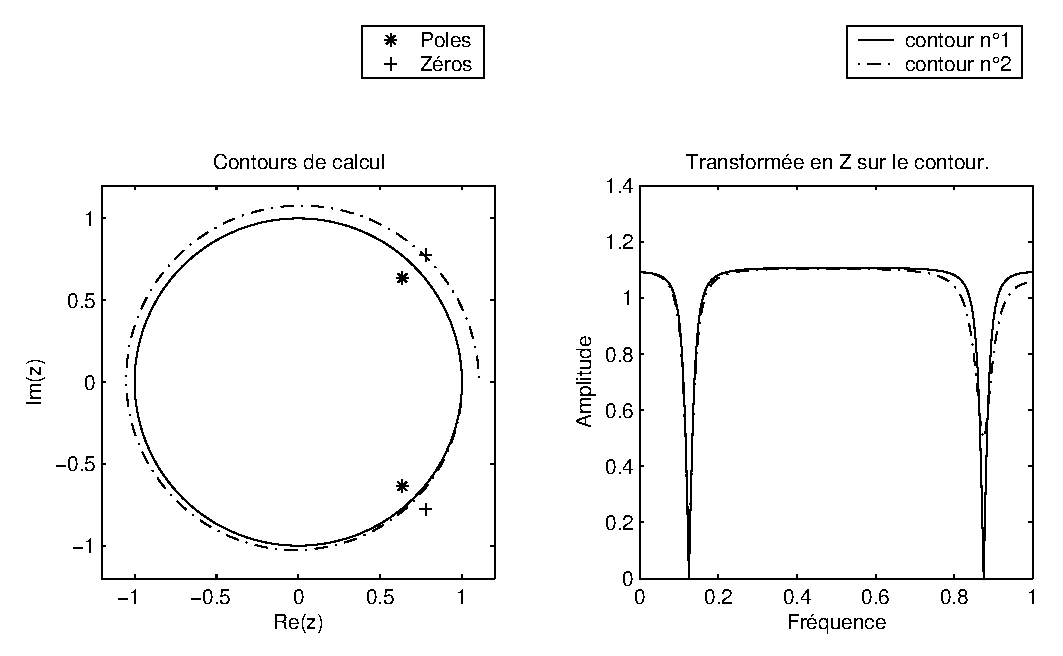
\includegraphics [scale = 0.6]{images/z-transform.eps}
    \end{center}
    \caption{Transformed into Z along two contours}
              \label{fig-z-transform}
\end{figure}
 
% ------------------------------------------------- -----
% ------------------------------------------------- -----
% sub-section - Applications to the discrete Fourier transform                            
% ------------------------------------------------- -----
% ------------------------------------------------- -----
\subsection{Applications to the discrete Fourier transform}
\label{sect2-applications-z-transform-tfd} 
 
 
This paragraph makes the connection between the vector Z transform and the DFT. In particular, we are going to see how this approximation makes it possible to perform DFT calculations in the case where the length $ N $ of the signals is not a composite number of the type $ N = 2^p $ (case where the FFT algorithm is very effective).
 
 
\index{Algorithm!chirp transform} \index{Chirp} We can indeed see the discrete Fourier transform as a particular case of vector Z transform. For that, we choose $ z = \omega_N \eqdef e^{\frac{2 \imath \pi}{N}} $ and we obtain, for a vector $ f \in \CC^N $,
\begin{equation*}
\Ff(f) = \Gg_{\omega_N} (f).
\end{equation*}
However, one of the strengths of the \textit{chirp transform} algorithm presented in the previous paragraph is that it can be applied to any positive integer $ N $. Unlike the FFT algorithm, it is not restricted to only integers $ N $ for which we know a \guill{good} factorization (the simplest example is $ N = 2^p $), as explained in Paragraph~\ref{sect2-transfo-cooley-tukey}. We can even apply the \textit{chirp transform} algorithm for transforms whose length $ N $ is a prime number, whereas in this case it is impossible to reduce the computation time by an FFT approach!Of course, this algorithm requires a number of additional calculations, among others: \begin{rs}
\item \index{Convolution!circular} \index{Convolution!acyclic} addition of zeros to transform acyclic convolution into circular convolution. In fact, we are going to calculate FFTs of length $ M = 2^k $ just after $ 2 N-1 $.
\item calculation of two FFTs (or even three taking into account the vector $ g $) to calculate a circular convolution.
\end{rs} However, in the case where we have to calculate a DFT of length $ N $ (and where we cannot replace these calculations by a larger transform), this algorithm constitutes an advantageous alternative compared to the calculation naive. However, it should be kept in mind that in a good number of applications, one can be satisfied with computing a transform at the frequencies $ \{k / N'\}_{k = -N' / 2}^{N'/ 2-1} $ rather than $ \{k / N \}_{k = -N / 2}^{N / 2-1} $, and therefore this approach is to be avoided!
 
\begin{rem}
The worst case that can arise for the \textit{chirp} algorithm for calculating a DFT is $ 2N-1 = 2^p + 1 $. We must indeed calculate 3 FFT of size $ 2^{p + 1} \approx 4N $ for the calculation of the convolution (we have $ N'= 2^{p + 1} $ and we must double the size because the convolution is not circular). We therefore see that we carry out about 12 times more calculations than for an FFT of size $ 2^p $ ...
\end{rem}
 
% ------------------------------------------------- -----
% ------------------------------------------------- -----
% ------------------------------------------------- -----
% section - Fractional Fourier transform                            
% ------------------------------------------------- -----
% ------------------------------------------------- -----
% ------------------------------------------------- -----
\section{Fractional Fourier transform}
% \addcontentsline{toc}{section}{Fractional Fourier transform}
\label{sect1-transforme-fourier-fractionionnaire} 
 
In this section, we will study the \textit{fractional Fourier transform}. It is simply a question of considering intermediate frequencies when evaluating the sum that defines the DFT. Certainly, we lose many properties of the discrete Fourier transform (convolution, inversion, etc.), since we no longer use the exponential characters $ e_n: k \mapsto e^{\frac{2 \imath \pi }{N} kn} $. However, we will see that we have a fast calculation algorithm, which makes this transform easy to use. A relatively complete presentation of the fractional Fourier transform is given in \cite{bailey-frac-trans}.
% ------------------------------------------------- -----
% ------------------------------------------------- -----
% sub-section - Definition and calculation algorithm                            
% ------------------------------------------------- -----
% ------------------------------------------------- -----
\subsection{Definition and calculation algorithm}
\label{sect2-trans-frac} 
 
 
\index{Fourier transform!fractional} Here is the definition, very natural, of this new transform.
 
\begin{defn}[Fractional Fourier transform]
\index{Fractional Fourier transform} Let $ \alpha \in \RR $. We define the \textit{fractional Fourier transform} $ G (f, \, \alpha) $ of a vector $ f \in \CC^N $ by
\begin{equation*}
\forall k \in \{0, \ldots, \, N-1 \}, \quad G (f, \, \alpha) [k] \eqdef \sum_{n = 0}^{N-1}{f [n] e^{- \alpha \frac{2 \imath \pi}{N} kn}}.
\end{equation*}
\end{defn}
 
 
\begin{rem}{(\upshape \textbf{Link with DFT}).} 
We see that if $ \alpha = 1 $, we find the discrete Fourier transform. For $ \alpha = -1 $, we find the inverse discrete Fourier transform (up to a factor of $ 1 / N $). It is in this sense that the fractional transform generalizes the usual TFD.
\end{rem}
 
 
 
In order to build a computational algorithm, we will make the link with the transform in Z, defined by the equation \eqref{eq-defn-z-transform-vector}. We indeed note that in the case where $ z = e^{\frac{2 \imath \alpha \pi}{N}} $, the two transforms coincide. By using the chirp transformation algorithm in Z, we will therefore be able to calculate the fractional Fourier transform quickly.
 
 
The fractional Fourier transform does not really have a simple intuitive meaning. We will see in the next paragraph that it allows to calculate intermediate values of the Fourier transform of a discrete signal. It will thus prove to be effective for analyzing signals whose periodicity is unknown. However, the fractional Fourier transform is not what one could call a partial transform, as we were able to define in Paragraph~\ref{sect2-eigenvalues-tfd}, and in the exercise \oldref{exo-transforme-partial-fourier}. Indeed, the composite of two fractional transforms with $ \alpha = \frac{1}{2} $ does not give back the classical Fourier transform.
 
 
The figure \figref{fig-transforme-fourier-fractionionnaire-1d} shows the fractional Fourier transforms $ G (f, \, \alpha) $ of a step function for several values of $ \alpha $. The exercise \oldref{exo-transforme-fourier-fractionionnaire-2d} proposes to calculate the fractional Fourier transforms of an image. \begin{figure}[ht]
    \begin{center}
    \includegraphics[scale=0.7]{images/transformee-fourier-fractionnaire-1d.png}
    \end{center}
    \caption{Fractional Fourier transforms of a 1D function}
              \label{fig-transforme-fourier-fractionionnaire-1d}
\end{figure}
 
% ------------------------------------------------- -----
% ------------------------------------------------- -----
% sub-section - Analysis of signals with non-integral periodicity                            
% ------------------------------------------------- -----
% ------------------------------------------------- -----
\subsection{Analysis of signals with non-integral periodicity}
\label{sect2-applications-trans-frac-periodicite} 
 
 
\index{Non-integer periodicity} \index{Sampling} \index{Signal} The discrete Fourier transform is a powerful tool for analyzing physical data collected by sensors or other more or less sophisticated methods. However, all this analysis made using the Fourier transform assumes that the recorded signal is periodic, and above all that its period is a divisor of the length over which the signal was sampled. However, in most applications, we are far from being able to know \textit{a priori} this period. In some cases, information is available on the value of this period. A good example is meteorological data. We know that the period of rotation of the earth around the sun is $ 365.2422 days. However, even in this favorable case, the data acquired is acquired at a rate of once a day, or $ 365 $ data per year. As a result, the signal spectrum is going to be unusually complicated, much more so than if we had been able to obtain exactly $ 365.2422 samples per year.
 
 
We are therefore faced with a double problem. \begin{rs}
\item How to determine, from a given spectrum, the true period of the signal?
\item Once this period is known, how to modify the original spectrum so that it corresponds to data sampled according to the correct period?
\end{rs} We need to build an algorithm that automates these two tasks, and does the math quickly. We will see that the use of the fractional Fourier transform and its fast algorithm solves this problem.
 
 
To get an idea of how to find the period, it is interesting to study what happens on a monochromatic sample, that is, on a sinusoid. Either the signal
\begin{equation*}
f = \left\{e^{\beta k \frac{2 \imath \pi}{N}} \right\}_{k = 0}^{N-1},
\end{equation*}
where $ \beta $ is a real number. If $ \beta $ is not an integer, we are in the presence of a signal that we know to be periodic (of period $ N / \beta $), but the sampling of which does not reflect the periodicity. The figure \figref{fig-spectrum-non-periodic-signal} shows the spectrum obtained for $ \beta = 4.63 $. We have plotted both the discrete Fourier transform and the continuous Fourier transform (which is approximated by adding a significant number of zeros at the end of the signal before calculating the DFT). 

\begin{figure}[ht]
    \begin{center}
    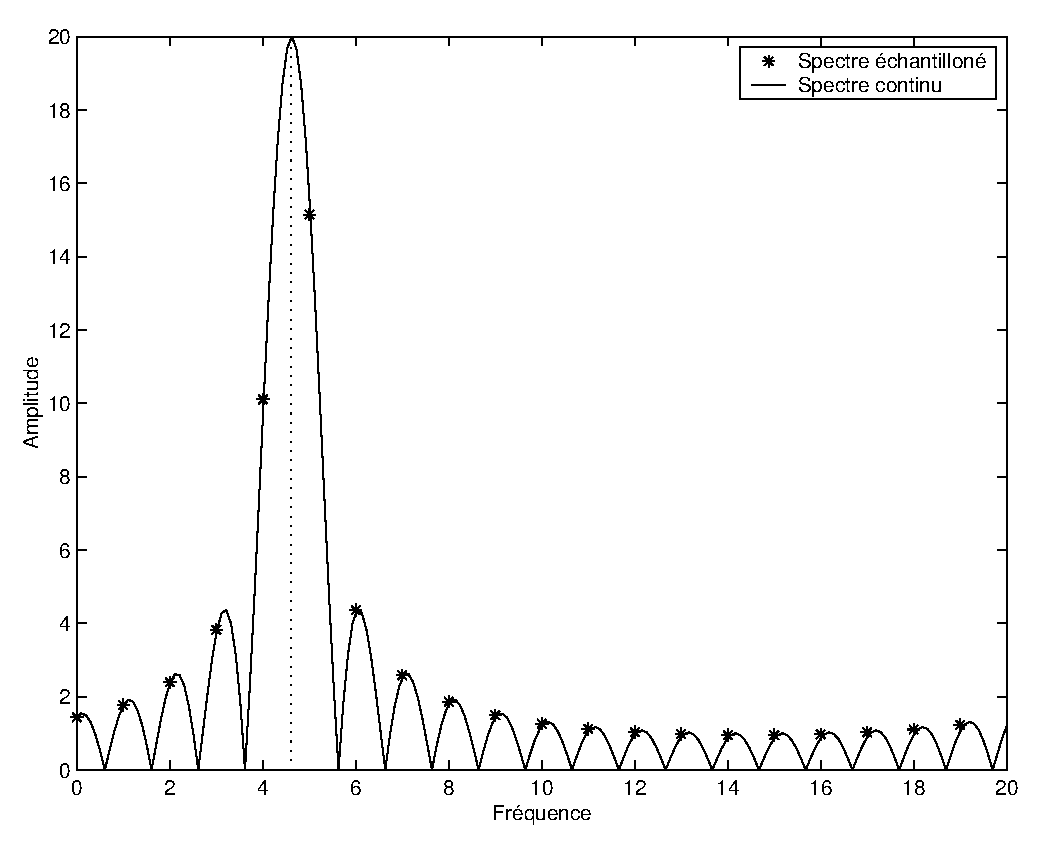
\includegraphics[scale=0.4]{images/spectre-signal-non-periodique.eps}
    \end{center}
    \caption{Spectrum of a badly sampled sinusoid}
              \label{fig-spectrum-non-periodic-signal}
\end{figure}

Although the spectrum is not equal to that which a monochromatic wave should have (we should obtain a single line placed at the frequency $ 4.63 $), it presents a maximum from which the values of the transform decrease. In the drawing, it is easy to determine the exact value of the abscissa of this maximum, which corresponds to the sought frequency and which allows us to determine the period. However, it is much too expensive to calculate the continuous Fourier transform to have a good approximate value of the period. Without knowing this continuous Fourier transform, we are nevertheless able to determine the period to within one unit. Here we see that this sought frequency is between $ 4 $ and $ 5 $. Let us denote by $ b $ the integer immediately less than $ \beta $. To calculate $ \beta $ with more precision, we will calculate in a finer way the spectrum of $ f $ in the interval $ [b, \, b + 1] $. Let $ \delta $ therefore be a subdivision step. We are looking for the value of the Fourier transform of $ f $ at the intermediate frequencies $ b, \, b + \delta, \ldots, \, b + m \delta \ge b + 1 $, which amounts to doing the calculation:
\begin{equation*}
\forall k \in \{0, \ldots, \, m \}, \quad \wh{f} (b + k \delta) = \sum_{n = 0}^{N-1}{f [n ] e^{- \frac{2 \imath \pi}{N} n (b + k \delta)}} = G (\wt{f}, \, \delta) [k],
\end{equation*}
where $ \wt{f} $ is the vector
\begin{equation*}
\wt{f} = \left\{f [n] e^{- \frac{2 \imath \pi}{N} nb} \right\}_{n = 0}^{N-1}.
\end{equation*}
The figure \figref{fig-transforme-fourier-fractionionnaire} (a) shows a periodic signal (noisy) whose sampling length is unfortunately not chosen to be multiple of the period. In figure (b), we can see the spectrum of this signal, which has a peak at $ b = $ 2. Figure (c) zooms in on the frequency window $ [2, \, 3] $, and we can see precisely that $ \beta = 2.23 $.
 
 
Now that we have precisely calculated the frequency $ \beta $ which determines the period, we would like to modify the spectrum so that this frequency $ \beta $ takes the place of a frequency actually calculated by the DFT, by the occurrence the frequency $ b $. We hope that the coefficients will decrease more quickly, as is the case with a well sampled monochromatic wave. Let $ \alpha = \frac{b}{\beta} $, which is slightly smaller than 1. Let $ r $ be the integer closest to $ N \alpha $. In order for the frequency $ \beta $ to become the frequency $ b $, we need to calculate a Fourier transform by multiplying the frequencies by $ \frac{1}{\alpha} $, which leads to calculate
\begin{equation*}
\forall k \in \{0, \ldots, \, r-1 \}, \quad F_k \eqdef \wh{f} \left(\frac{k}{\alpha} \right) = \sum_{n = 0}^{r-1}{f [n] e^{- \frac{2 \imath \pi}{N \alpha} kn}} = G \left(f, \, \frac{r}{N \alpha} \right) [k],
\end{equation*}
where care must be taken to complete the vector $ f $ with zeros so that it reaches the length $ r $. In the case where $ N \alpha = r $ is an integer, and the signal $ f $ is monochromatic as we have already defined, we obtain
\begin{equation*}
\forall k \in \{0, \ldots, \, r-1 \}, \quad \wh{f} \left(\frac{k}{\alpha} \right) = \sum_{n = 0}^{r-1}{e^{\frac{2 \imath \pi}{N} \beta n} e^{- \frac{2 \imath \pi}{r} nk}} = r \delta_b^k.
\end{equation*}
We therefore obtain the desired result, namely a perfect correction of the spectrum. If $ N \alpha $ is not an integer, the correction is however not perfect; we can calculate the error obtained for a monochromatic wave:
\begin{align*}
\forall k \in \{0, \ldots, \, r-1 \}, \; k \neq b, \quad F_k \eqdef \left| \wh{f} \left(\frac{k}{\alpha} \right) \right| & = \left| \frac{1 - e^{- \frac{2 \imath \pi}{N \alpha} n (bk)}}{1 - e^{- \frac{2 \imath \pi}{N \alpha} (bk)}} \right| \\
& = \left| \frac{sin \left(\frac{\pi s (bk)}{N \alpha} \right)}{\sin \left(\frac{\pi (bk)}{N \alpha} \right)} \right|,
\end{align*}
where we noted $ s \eqdef r - N \alpha $. By noting that $ | s | <\frac{1}{2} $, we see that \begin{rs}
\item we have $ F_b = r $, as in the case where $ N \alpha $ is integer.
\item when $ k $ is close to $ b $, in the first order, we have $ | F_k | \equiv | s | $ which is bounded by $ \frac{1}{2} $, so much smaller than $ F_b $.
\item When $ k $ is far from $ b $, on the other hand, the situation is less favorable (the denominator of $ | F_k | $ may become small). However, using the fact that
\begin{equation*}
\forall x \in [0, \pi / 2], \quad \frac{2 x}{\pi} \leq \sin (x) \leq x
\end{equation*}
we show that $ | F_k | $ remains bounded by $ \frac{N}{\pi \beta} $ or $ \frac{N}{\pi (N- \beta)} $.
\end{rs} In the case where the signal is not monochromatic, the decrease will of course be weaker, and the improvement less visible. Figure \figref{fig-transforme-fourier-fractionionnaire} (d) shows the effect of this frequency adjustment, and we observe a marked decrease in the values of the transform outside the peak at the frequency $ 2 $. We have obtained a frequency representation of the analyzed function that is much more efficient and able to be used for subsequent processing. \begin{figure}[ht]
    \begin{center}
    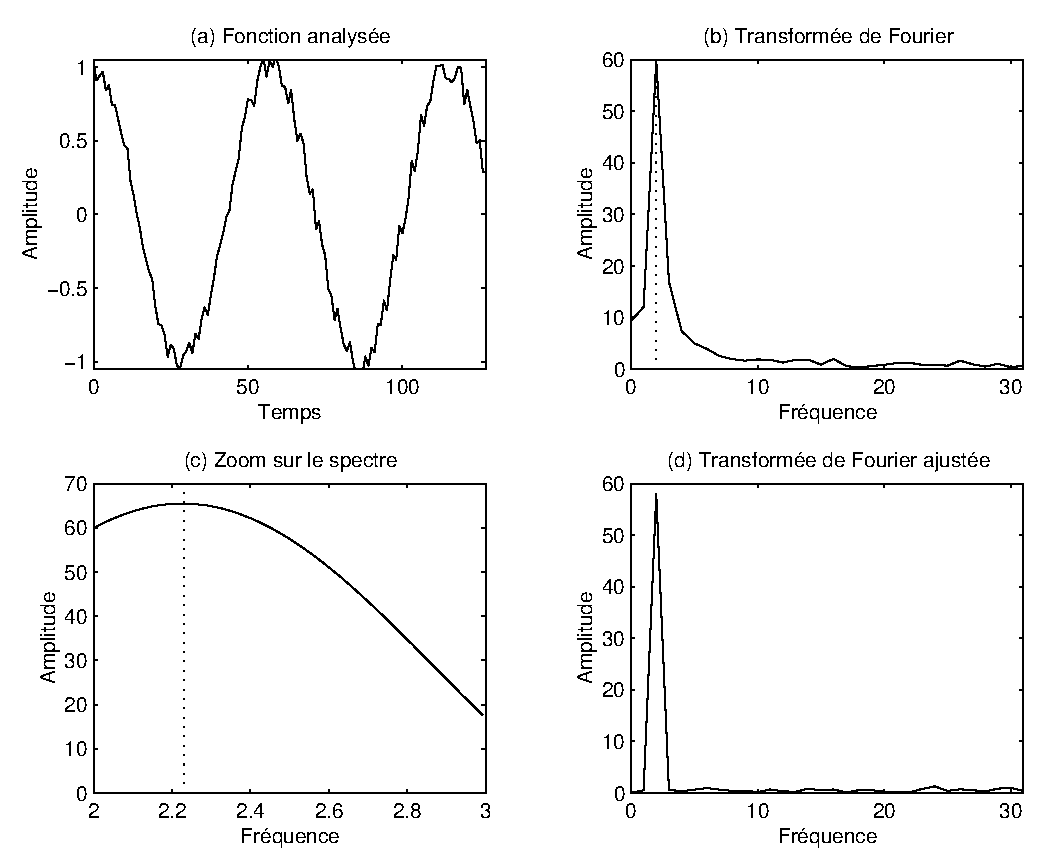
\includegraphics[scale=0.6]{images/transformee-fourier-fractionnaire.eps}
    \end{center}
    \caption{Spectrum adjustment by fractional Fourier transform}
              \label{fig-transforme-fourier-fractionionnaire}
\end{figure}
 
% ------------------------------------------------- -----
% ------------------------------------------------- -----
% ------------------------------------------------- -----
% section - Exercises                            
% ------------------------------------------------- -----
% ------------------------------------------------- -----
% ------------------------------------------------- -----
\section{Exercises}
% \addcontentsline{toc}{section}{Exercises}
\label{sect1-ext-trans-fourier-exercises} 
 
 
 
\begin{exo}[Eigenvectors and Hartley transform]
\label{exo-eigenvectors-transfo-hartley}
 
\index{Eigenvalue} \index{Eigenvector} What are the eigenvalues of the Hartley transform defined in Section~\ref{sect1-trans-hartley}? Inspired by the construction of Paragraph~\ref{sect2-eigenvalues-tfd}, propose a method to obtain eigenvectors for each of the eigenvalues. Based on what was done in the paragraph, deduce the construction of an intermediate Hartley transform $ \Hh^\lambda $. The figure \figref{fig-transfo-hartley-interm} shows different intermediate transforms. We can make the comparison with the figure \figref{fig-root-interm-tfd}. \begin{figure}[ht]
    \begin{center}
    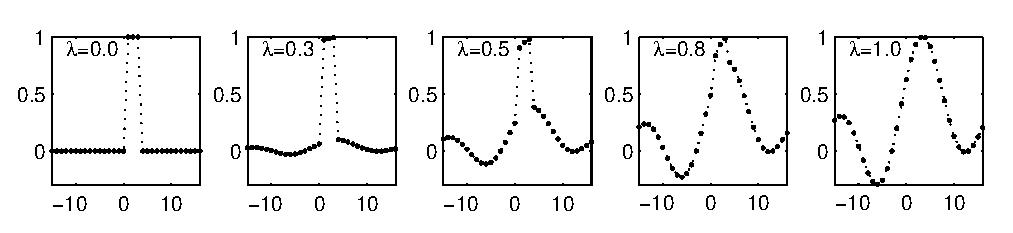
\includegraphics[scale=0.7]{images/transfo-hartley-interm.eps}
    \end{center}
    \caption{Real parts of intermediate transforms $ \Hh^\lambda (f) $ for $ \lambda \in [0,1] $}
              \label{fig-transfo-hartley-interm}
\end{figure}
\end{exo}
 
 
\begin{exo}[Generalized Hartley transform]
\label{exo-transfo-hartley-generalisee}
 
\index{Generalized Hartley transform!} Noting that
\begin{equation}
\label{eq-factorization-case}
\cas (x) = \sqrt{2} \cos \left(x - \frac{\pi}{4} \right),
\end{equation}
we can define, for $ f \in \RR^N $, a Hartley transform generalized by
\begin{equation*}
\forall n \in \{0, \ldots, \, N-1 \}, \quad \Hh_{\lambda} (f) [n] \eqdef \sum_{k = 0}^{n-1}{f [k] \cos \left(\frac{2 \pi}{N} nk + \lambda \right)},
\end{equation*}
where $ \lambda $ is an actual parameter in $ [0, \pi [$. For $ \lambda \notin \left\{0, \, \frac{\pi}{2} \right\} $, show that this transformation is bijective, and that its inverse is given by
\begin{equation}
\label{eq-inverse-hartley-generalized}
(\Hh_\lambda)^{-1} = \frac{2}{\sin (2 \lambda)} \Hh_{\frac{\pi}{2} - \lambda}.
\end{equation}
Figure \figref{fig-transforme-hartley-generalized} shows the generalized transform of the triangular signal in figure \figref{fig-comparison-fht-fft} (left), for $ \lambda $ varying between $ 0 $ and $ 2 \pi $. 

\begin{figure}[ht] 
    \begin{center}
    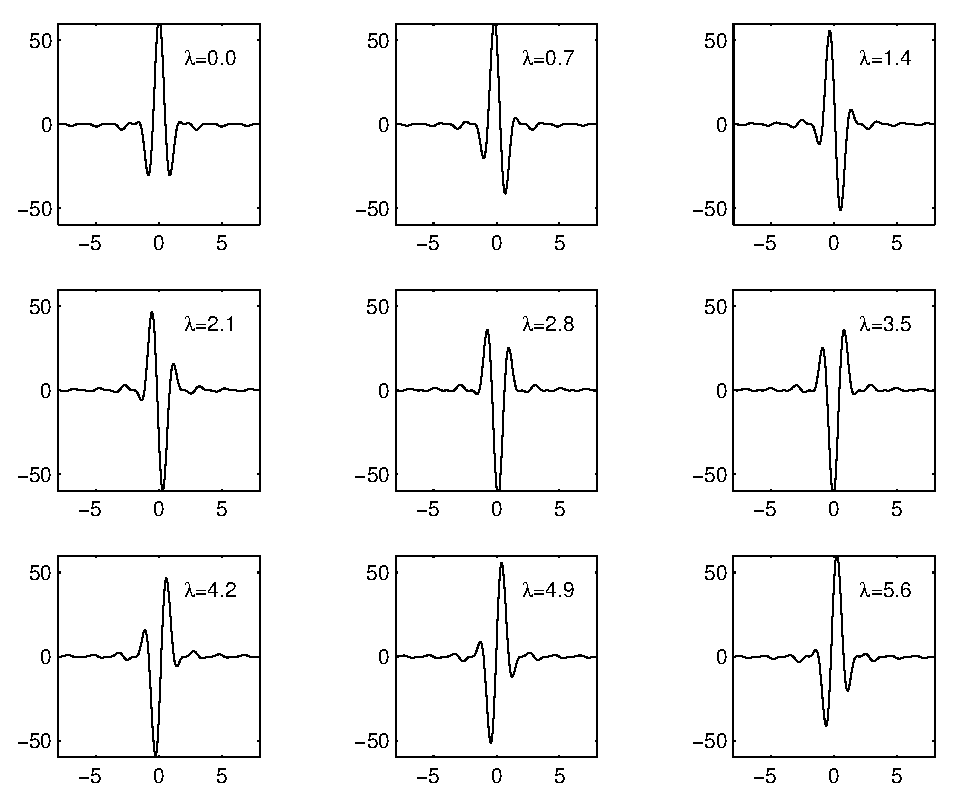
\includegraphics[scale=0.7]{images/transformee-hartley-generalisee.eps}
    \end{center}
    \caption{Generalized Hartley transform for different values of $ \lambda $}
              \label{fig-transforme-hartley-generalized}
\end{figure}
\end{exo}
 
 
\begin{exo}[Interpolation and Hartley transform]
\label{exo-interpolation-transfo-hartley}
 
\index{Zero padding} \index{Interpolation} In the exercise \oldref{exo-interpolation-trigonometric}, we saw how we can interpolate a sampled signal thanks to the discrete Fourier transform. Still using the zero padding technique, explain why the discrete Hartley transform also allows you to interpolate sampled values. Show that in fact the interpolations obtained by Fourier and by Hartley are the same.
\end{exo}
 
 
\begin{exo}[Hartley transform 2D]
\label{exo-transfo-hartley-2d}
 
\index{2D Hartley transform} \index{Inversion!formula} Let $ f \in \RR^{N_1 \times N_2} $. We define its two-dimensional Hartley transform $ \Hh (f) $ by
\begin{equation*}
\Hh (f) [n_1, \, n_2] \eqdef \sum_{k_1 = 0}^{N_1-1}{\sum_{k_2 = 0}^{N_2-1}{f [k_1, \, k_2] \cas \left(\frac{2 \pi}{N_1} k_1 n_1 \right) \cas \left(\frac{2 \pi}{N_2} k_2 n_2 \right)}},
\end{equation*}
where $ n_1 \in \{0, \ldots, \, N_1-1 \} $ and $ n_2 \in \{0, \ldots, \, N_2-1 \} $. Show that we have the following inversion formula:
\begin{equation*}
f = \frac{1}{N_1 N_2} \Hh (\Hh (f)).
\end{equation*}
How to quickly calculate this transform using the FHT algorithm?
\end{exo}
 
 
\begin{exo}[Hartley transform and finite fields]
\label{exo-transfo-hartley-corps-finis}
 
\index{Hartley transform!on a finite field} Extend the definition of the \textit{Hartley transform} within the framework of finite fields (then rings in which we have a root \ordin{n}{ième} main). If $ \zeta $ represents a \ordin{n}{ith} root of the unit, we can use $ \frac{\zeta^2 + 1}{2 \zeta} $ to replace $ \cos \left(\frac{2 \pi}{n} \right) $. Write the corresponding \textit{FHT} algorithm.
\end{exo}
 
 
\begin{exo}[Chirp transformation and Toeplitz matrices]
\label{exo-chirp-transform-toeplitz}
 
\index{Matrix!of Toeplitz} \index{Chirp} In this exercise, we use the description of the chirp algorithm for the calculation of the Z transform, in order to find a matrix formulation. Recall the definition of the chirp algorithm. It consists in calculating the transform in Z of a vector $ f \in \CC^N $ via a vector $ \{y [n] \}_{n = 0}^{N-1} $ defined by
\begin{equation*}
\forall n \in \{0, \ldots, \, N-1 \}, \quad y [n] \eqdef z^{\frac{n^2}{2}} \Gg_z (f) [n] = \sum_{n = 0}^{N-1}{h [k] g [nk]},
\end{equation*}
where we noted
\begin{equation*}
\forall k \in \{0, \ldots, \, N-1 \}, \quad h [k] \eqdef f [k] z^{- \frac{k^2}{2}},
\end{equation*}
and
\begin{equation*}
\forall k \in \{- N + 1, \, N-1 \}, \quad g [k] \eqdef z^{- \frac{k^2}{2}}.
\end{equation*}
\begin{enumerate}
\item Show that $ y $ can be calculated as a matrix product $ y = G h $, where $ G $ is what we call a matrix of \textit{Toeplitz}, i.e. a matrix constant along each of its diagonals. For example, show that for $ N = 3 $, we have
\begin{equation*}
G = \begin{pmatrix} g [0] & g [1] & g [2] \\g [1] & g [0] & g [1] \\g [2] & g [1] & g [0] \end{pmatrix}.
\end{equation*}
 
\item In general, a Toeplitz matrix $ T $ of size $ m \times n $ is written
\begin{equation*}
T \eqdef \begin{pmatrix} t_{m-1} & t_{m} & \ldots & t_{m + n-2} \\t_{m-2} & t_{m-1} & \ldots & t_{m + n-3} \\\vdots & \ldots & \ldots & \vdots \\t_0 & \ldots & \ldots & t_{m-1} \end{pmatrix}.
\end{equation*}
It is therefore entirely determined by its first column, which we denote in the form $ t_c \eqdef \transp{(t_0, \ldots, \, t_{n-1})} $ and its first row denoted $ t_{l} \eqdef \transp{(t_m, \ldots, \, t_{m + n-2})} $ (we do not take the element $ t_{m-1} $). We consider the vector
\begin{equation*}
c \eqdef \transp{(t_c, \, 0, \ldots, \, 0, \, t_l)} \in \CC^{M}.
\end{equation*}
\index{Matrix!circulating} where $ M $ is the power of two immediately after $ n + m-1 $. We denote by $ C $ circulating matrix associated with $ c $, as defined in exercise \oldref{exo-circulating-matrix}. Where can we find the matrix $ T $ inside the matrix $ C $? How to calculate a product $ T x $, where $ x \in \CC^n $, using the matrix $ C $? Deduce an algorithm allowing to calculate $ C x $ quickly, using the FFT algorithm.
\item Apply the previous construction to the $ G $ matrix. Show for example that in the case $ N = 3 $, we obtain the following matrix $ C $:
\begin{equation*}
C = \begin{pmatrix} g [0] & g [1] & g [2] & 0 & 0 & 0 & g [2] & g [1] \\g [1] & g [0] & g [1] & g [2] & 0 & 0 & 0 & g [2] \\g [2] & g [1] & g [0] & g [1] & g [2] & 0 & 0 & 0 \\0 & g [2] & g [1] & g [0] & g [1] & g [2] & 0 & 0 \\0 & 0 & g [2] & g [1] & g [0] & g [1] & g [2] & 0 \\0 & 0 & 0 & g [2] & g [1] & g [0] & g [1] & g [2] \\g [2] & 0 & 0 & 0 & g [2] & g [1] & g [0] & g [1] \\g [1] & g [2] & 0 & 0 & 0 & g [2 ] & g [1] & g [0] \end{pmatrix}.
\end{equation*}
Deduce an algorithm allowing to calculate $ y $, then $ \Gg_z (f) $ quickly.
\end{enumerate}
\end{exo}
 
 
\begin{exo}[Quadrature methods and recursive filters]
\label{exo-meth-quadratures-recursive-filter}
 
\index{Method!of quadrature} \index{Method!of rectangles} \index{Method!of trapezoids} \index{Method!of Simpson} \index{Calculation!of integral} We consider an integrating circuit, which connects the input voltage $ x (t) $ and output voltage $ y (t) $ by the equation
\begin{equation*}
y (t) = \int_{0}^{t}{x (\tau) \d \tau}.
\end{equation*}
What is the transfer function of this filter in the Laplace domain? We want, from this analog filter, to create a digital recursive filter. We consider the following quadrature methods, for a function $ f: \RR \rightarrow \RR $ continue:
\begin{align}
\label{eq-defn-meth-quadrature}
(M_0) \quad \quad \int_0^1{f(t) \d t} & \approx f(0), \\
(M_1) \quad \quad \int_0^1{f(t) \d t} & \approx \frac{1}{2} \left(f(0) + f(1) \right), \\
(M_2) \quad \quad \int_0^1{f(t) \d t} & \approx \frac{1}{6} f(0) + \frac{2}{3} f(1/2) + \frac{1}{6} f(1).
\end{align}
These methods are called the \textit{rectangles on the left} method, the \textit{trapezoids} method, and the \textit{Simpson} method, respectively. Considering a discretization of the signals $ x $ and $ y $ of steps $ \Delta $, give the recurrence equations obtained by using each of the three methods. What are the associated transfer functions (for the Z transform)?
\end{exo}
 
 
\begin{exo}[Spline and recursive filters]
\label{exo-calcul-spline-iir}
 
\index{Spline!cubic} \index{Filter!recursive} We use the notations of the exercise \oldref{exo-spline-filtering}. This is to explain how we can calculate the interpolation coefficients $ c [k] $ by means of a recursive filter. We will mainly focus on the example of cubic splines, and we leave it to the reader to practice on other examples, then to generalize the method. To use an expression of $ \beta^n_d $, we can refer to the article of \nompropre{Unser}{\upshape \cite{unser-spline}}. \begin{enumerate}
\item Calculate $ \beta^3_d $, then show that its transform in Z is worth
\begin{equation*}
\Zz (\beta^3_d) (z) = \frac{z + 4 + z^{-1}}{6}.
\end{equation*}
 
\item \index{Decomposition!into simple elements} \index{Simple element} Recall that we have $ c = \Phi^3_d * u_d $, where $ \Phi^3_d $ is defined by $ \wh{\Phi^3_d} = 1 / \wh{\beta^3_d} $. Decompose the rational fraction $ \Zz (\Phi^3_d) $ into simple elements. How can we calculate the coefficients $ c $ of the indirect interpolation using two recursive filters?
\item We assume that we know the signal $ u_d [k] $ for $ k \in \{0, \ldots, \, K-1 \} $. Show that we can organize the calculations of $ c $ as follows:
\begin{equation*}
\left\{\begin{array}{ll} \forall k \in \{1, \ldots, \, K-1 \}, & c^+ [k] = u_d [k] + b_1 c^+ [ k-1] \\\forall k \in \{0, \ldots, \, K-2 \}, & c^- [k] = u_d [k] + b_1 c^- [k + 1] \\\forall k \in \{0, \ldots, \, K-1 \}, & c [k] = b_0 (c^+ [k] + c^- [k] - u_d [k]) \end{array} \right. .
\end{equation*}
We will specify the values of the constants $ b_0 $ and $ b_1 $. What values should $ c^+ [0] $ and $ c^- [K-1] $ be given? It will be possible for example to ensure that the produced signal can be prolonged by mirror symmetry in $ K-1 $ and $ 0 $ (to avoid discontinuities).
\item Resume the two previous questions by exploiting a product decomposition of the form
\begin{equation*}
\Zz (\Phi^3_d) = \frac{A}{(1- \alpha z^{-1}) (1- \alpha z)}.
\end{equation*}
\end{enumerate}
\end{exo}
 
 
\begin{exo}[Chirp transformation and finite field]
\label{exo-chirp-transform-finis-corps}
 
\index{Chirp} \index{Finite field} Let $ p $ be a prime number. We denote by $ g $ a generator of the group $ \FF_p^* $. \\A function $ f: \{0, \ldots, \, p-1 \} \rightarrow \CC $ will be considered as a function defined on $ \FF_p $. Show that we can write the Fourier transform of $ f $ as follows:
\begin{equation*}
\forall b \in \{0, \ldots, \, p-2 \}, \quad \wh{f} (g^{- b}) = f(0) + \sum_{a = 0}^{p-2}{f(g^a) \omega_p^{-g^{ab}}},
\end{equation*}
where $ \omega_p = e^{\frac{2 \imath \pi}{p}} $. Deduce that we can calculate the Fourier transform of $ f $ using a convolution on $ \ZZ/(p-1) \ZZ $. Specify the vectors involved, and implement this algorithm.
\end{exo}
 
 
\begin{exo}[Calculations approximated by fractional Fourier transform]
\label{exo-calcul-approaches-transfo-frac}
 
\index{Calculus!approximate} \index{Fourier transform!fractional} \index{Sampling} Let a continuous function $ f: \RR \rightarrow \RR $ be assumed to be supported in $ [- a / 2, \, a / 2] $. We have a regular sampling $ f [k] = f(x_k) $ with $ x_k = f((kN / 2) a / N) $ for $ k = 0, \ldots, \, N-1 $. \begin{enumerate}
\item We want to evaluate the continuous Fourier transform of $ f $ around a frequency $ \zeta $, more precisely at the points $ y_k = \zeta + \frac{2 \pi}{a} (kN / 2) \gamma $, where $ \gamma $ is the desired precision. If we want to calculate the $ \wh{f} (x_k) $ using the FFT algorithm, what is the size of the transform to calculate (we will assume that $ \gamma \in \QQ $ )? Show that we can perform this calculation more economically using the fractional Fourier transform.
\item \index{Simpson's!method} We now want to increase the precision of the calculations. Using the Simpson quadrature method (exercise \oldref{exo-meth-quadratures-recursive-filter}, method $ (M_2) $), explain how to modify the method of the previous question.
\end{enumerate}
\end{exo}
 
 
\begin{exo}[Fractional Fourier transform of an image]
\label{exo-transforme-fourier-fractionionnaire-2d}
 
Propose a 2D fractional Fourier transform which extends the 1D transform by tensor product (we can use the construction of the 2D Hartley transform, exercise \oldref{exo-transfo-hartley-2d}). Write the corresponding \Matlab{} function, and test the transform on several images. The figure \figref{fig-transforme-fourier-fractionionnaire-2d} shows the transforms of the indicator function of a disk.
 
\begin{figure}[ht] 
    \begin{center}
    \includegraphics[scale=0.7]{images/transformee-fourier-fractionnaire-2d}
    \end{center}
    \caption{Fractional Fourier transforms of a 2D function}
              \label{fig-transforme-fourier-fractionionnaire-2d}
\end{figure}
\end{exo}
 